\documentclass[twocolumn]{article}
\usepackage[utf8]{inputenc}

\usepackage{geometry}

\usepackage{fancyhdr}
% \usepackage{fullpage}
\usepackage{lscape}

% \usepackage{booktabs}
% \usepackage{verbatim}

% \usepackage{algpseudocode}
% \usepackage{algorithm}

% \usepackage{amsmath, amsfonts, amsthm, bm}
\usepackage{hyperref}
\usepackage{cleveref}

\usepackage{tikz}
\usepackage{tikz-3dplot} 
\usetikzlibrary{backgrounds,decorations.pathreplacing}
\usetikzlibrary{calc}
\usetikzlibrary{matrix}
\usetikzlibrary{backgrounds}
\usetikzlibrary{shapes}
\usetikzlibrary{positioning}

\usepackage{graphicx}
\usepackage{subcaption}

% \usepackage[inline]{enumitem}

% \usepackage{todonotes}
% \usepackage[framemethod=tikz]{mdframed}

\newcommand\grid[1]{
  \pgfmathsetmacro\size{#1}
  \draw[step=1,black,thin] (0,0) grid (\size-1,\size-1);
  \draw[step=\size-1,black,ultra thick] (0,0) grid (\size-1,\size-1);
}

\newcommand\xlabels[2]{
  \foreach \label [count=\i] in #2 {
    \node at (\i-1,-0.5) {\texttt{\label}};
    \node at (\i-1,#1-0.5) {\texttt{\label}};

    \ifnum \i=#1
      \breakforeach
    \fi
  }
}

\newcommand\ylabels[2]{
  \foreach \label [count=\i] in #2 {
    \node at (-0.5,#1-\i) {\texttt{\label}};
    \node at (#1-0.5,#1-\i) {\texttt{\label}};

    \ifnum \i=#1
      \breakforeach
    \fi
  }
}

\newcommand\letterlabels{A,...,Z}
\newcommand\numberlabels{1,...,19}
\newcommand\musiclabels{do,re,mi,fa,so,la,ti}

\newcommand\upperboard[1]{
  \grid{#1}
  \xlabels{#1}{\numberlabels}
  \ylabels{#1}{\musiclabels}
}

\newcommand\numberboard[1]{
  \grid{#1}
  \xlabels{#1}{\musiclabels}
  \ylabels{#1}{\letterlabels}
}

\newcommand\lowerboard[1]{
  \grid{#1}
  \xlabels{#1}{\letterlabels}
  \ylabels{#1}{\numberlabels}
}

\title{Multiverse Go}
% \author{}
\date{}

\begin{document}
\maketitle

\pagestyle{empty}

\section{Rules}

Multiverse go is a variant similar but distinct from 3D go.  Like 3D go, it is
played on a 3D goban.  However, the rules concerning stone liberties are
different.
%
The game is played on a 3D goban;  in this document we will use the $5\times
5\times 5$ grid as an example.  Rather than seeing it as a single $5 \times
5\times 5$ game of go, it should be seen as $15$ separate (but connected)
$5\times 5$ games.  Each 2D ``slice'' of the 3D goban represents a separate
``flat'' game.  In practice, when each move in the $5\times 5\times 5$ goban
corresponds to $3$ moves and $12$ passes in the $5\times 5$ ``slice'' gobans.

Each intersection can be identified by using 3D coordinates which range from
$\texttt{A1do}$ to $\texttt{E5so}$ (see \cref{fig:goban}), where
%
\begin{itemize}
  %
  \item the first axis uses $\texttt{A}$, $\texttt{B}$, $\texttt{C}$,
    $\texttt{D}$, $\texttt{E}$, etc.;
  %
  \item the second axis uses $\texttt{1}$, $\texttt{2}$, $\texttt{3}$,
    $\texttt{4}$, $\texttt{5}$, etc.; and
  %
  \item the third axis uses $\texttt{do}$, $\texttt{re}$, $\texttt{mi}$,
    $\texttt{fa}$, $\texttt{so}$, etc.
  %
\end{itemize}


These 3D coordinates uniquely identify both the 2D ``slice'' gobans in which
the moves are being played, and the coordinates within those ``slice'' gobans.
%
Each 2D board has a unique name;  in $5\times 5\times 5$ multiverse go, the
names are 
%
\texttt{A}, \texttt{B}, \texttt{C}, \texttt{D}, \texttt{E},
%
\texttt{1}, \texttt{2}, \texttt{3}, \texttt{4}, \texttt{5},
%
\texttt{do}, \texttt{re}, \texttt{mi}, \texttt{fa}, and \texttt{so}.
%
As an example, move \texttt{B4mi} represents the following ``flat'' coordinates:
%
\begin{itemize}
  %
  \item Move \texttt{4mi} on board \texttt{B};
  %
  \item Move \texttt{Bmi} on board \texttt{4}; and
  %
  \item Move \texttt{B4} on board \texttt{mi}.
  %
\end{itemize}

\tdplotsetmaincoords{60}{125}
%
\tdplotsetrotatedcoords{0}{0}{0} %<- rotate around (z,y,z)
%
\begin{figure}[t!]
  %
  \centering
  %
  \begin{tikzpicture}[scale=2,tdplot_rotated_coords,
                      cube/.style={very thick,black},
                      grid/.style={very thin,gray},
                      axis/.style={black,thick}]

    \draw[axis,tdplot_main_coords]
      (2,2.1,0) node[anchor=north west] {\texttt{A}}
      -- (1,2.1,0) node[anchor=north west] {\texttt{B}}
      -- (0,2.1,0) node[anchor=north west] {\texttt{C}};

    \draw[axis,tdplot_main_coords]
      (2.1,0,0) node[anchor=north east] {\texttt{1}}
      -- (2.1,1,0) node[anchor=north east] {\texttt{2}}
      -- (2.1,2,0) node[anchor=north east] {\texttt{3}};

    \draw[axis,tdplot_main_coords]
      (2,-0.1,2) node[anchor=east] {\texttt{do}}
      -- (2,-0.1,1) node[anchor=east] {\texttt{re}}
      -- (2,-0.1,0) node[anchor=east] {\texttt{mi}};

    %draw the top and bottom of the cube
    \draw[cube,fill=blue!5] (0,0,0) -- (0,2,0) -- (2,2,0) -- (2,0,0) -- cycle;

    %draw the top and bottom of the cube
    \draw[cube,fill=red!5] (0,0,0) -- (0,2,0) -- (0,2,2) -- (0,0,2) -- cycle;

    %draw the top and bottom of the cube
    \draw[cube,fill=green!5] (0,0,0) -- (2,0,0) -- (2,0,2) -- (0,0,2) -- cycle;

    \foreach \x in {0,...,2}
       \foreach \y in {0,...,2}
          \foreach \z in {0,...,2}{
               %#####################################################
               \ifthenelse{  \lengthtest{\x pt < 2pt}  }
               {
                 % True
                    \draw [black]   (\x,\y,\z) -- (\x+1,\y,\z);
               }
               {% False
               }
               %#####################################################
               \ifthenelse{  \lengthtest{\y pt < 2pt}  }
               {
                 % True
                    \draw [black]   (\x,\y,\z) -- (\x,\y+1,\z);
               }
               {% False
               }
               %#####################################################
               \ifthenelse{  \lengthtest{\z pt < 2pt}  }
               {
                 % True
                    \draw [black]   (\x,\y,\z) -- (\x,\y,\z+1);
               }
               {% False
               }
               \shade[axis,ball color=black] (\x,\y,\z) circle (0.05cm);
    }
    %
  \end{tikzpicture}
  %
  \caption{A $3\times 3\times 3$ goban and the 3D coordinate system.}\label{fig:goban}
  %
\end{figure}

\newgeometry{margin=0cm,includeheadfoot}
\onecolumn

\begin{center}
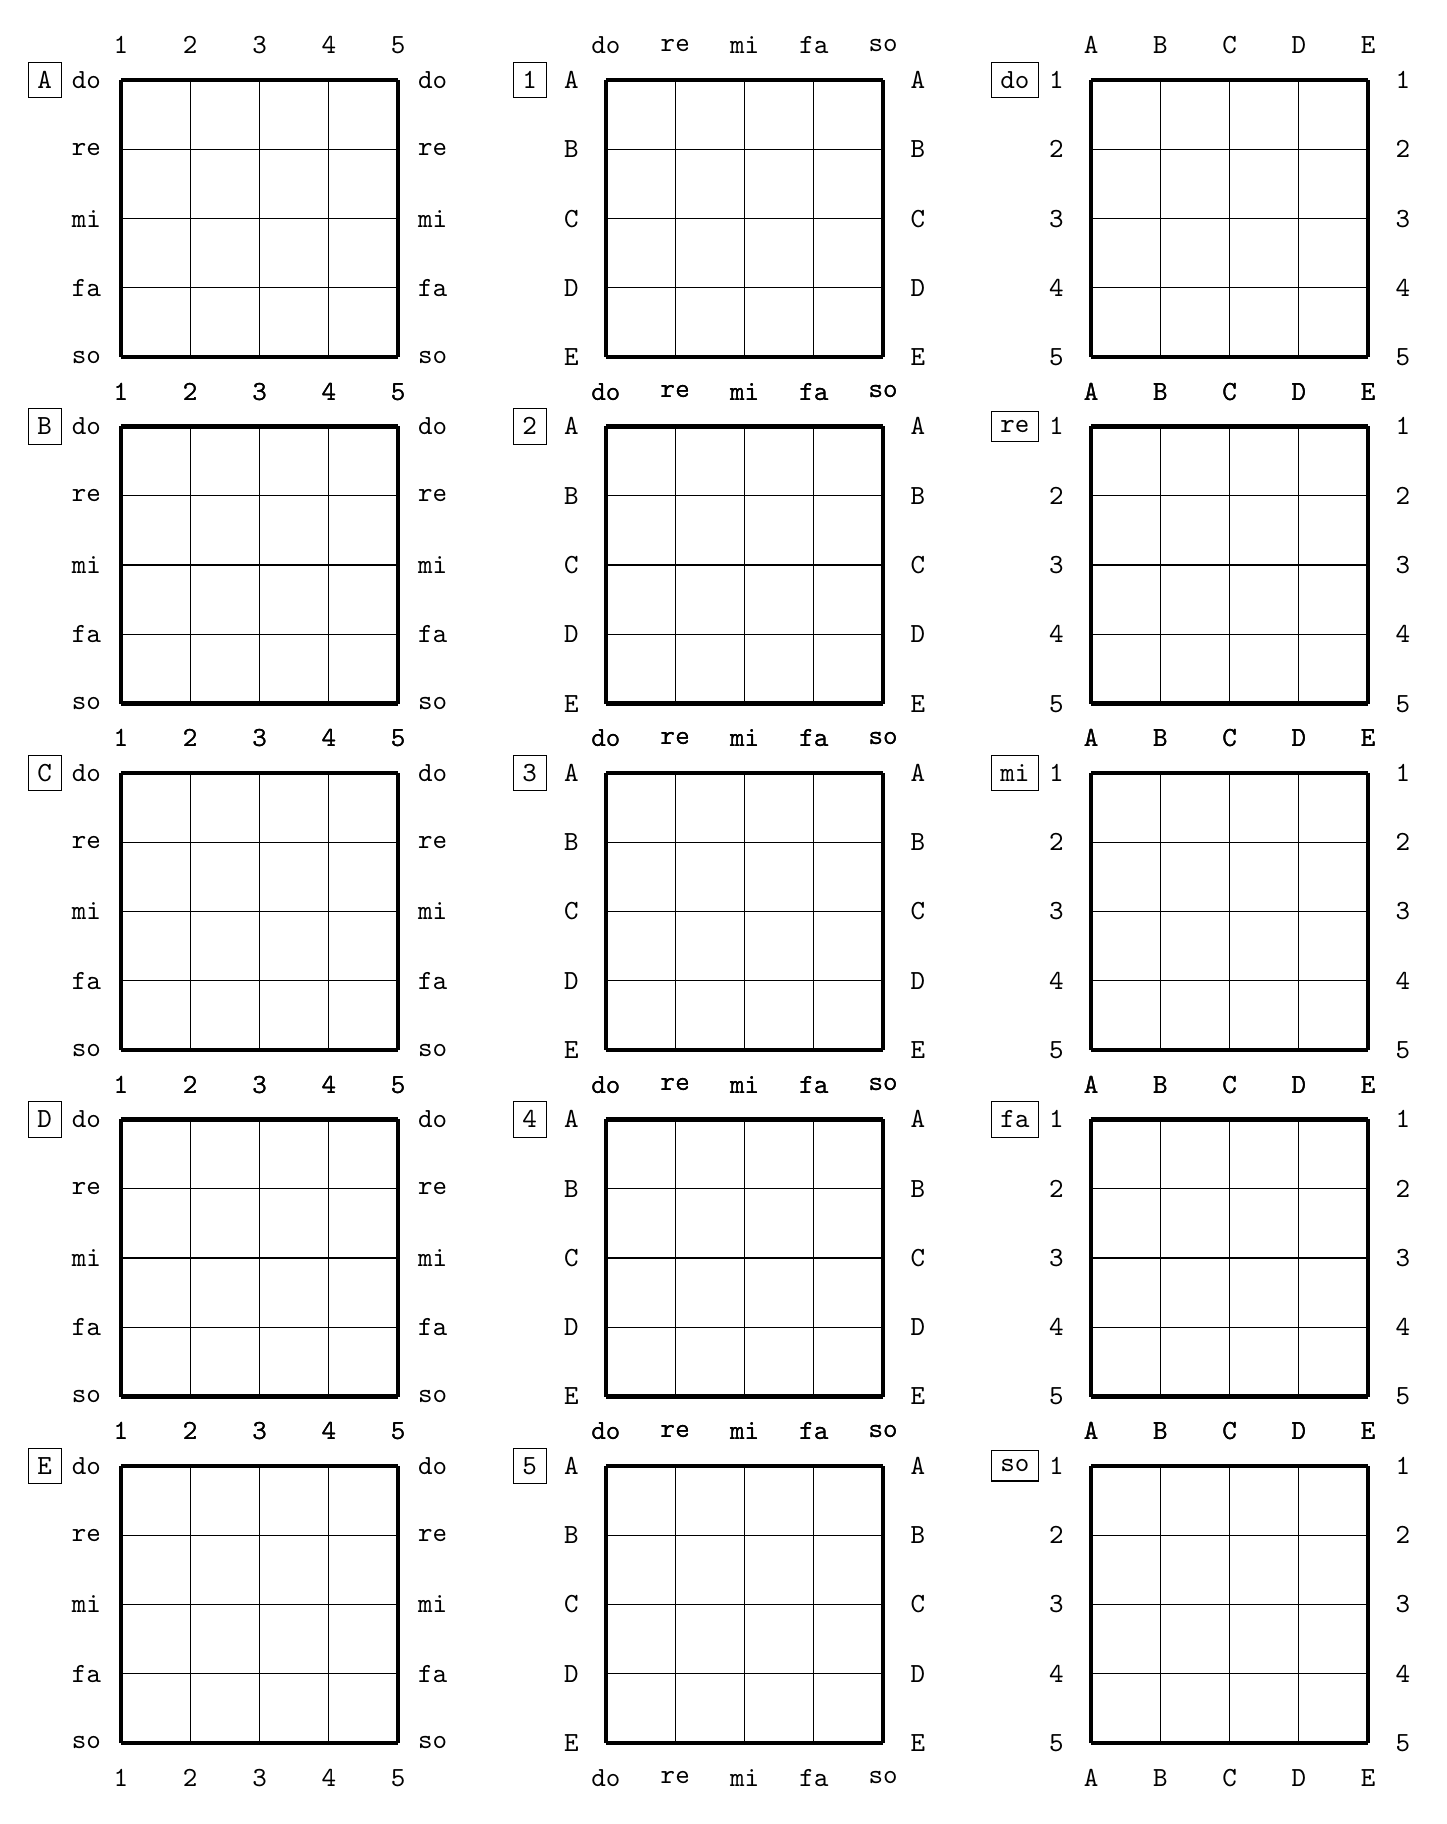
\begin{tikzpicture}
  %
  \newcommand\size{5}
  \begin{scope}[scale=1.1]

    \foreach \name [count=\i] in \letterlabels {
      \begin{scope}[scale=0.8,yshift=-\i*\size cm]

        \begin{scope}[shift={(-1.1,\size - 1)}]
          \node[draw] at (0,0) {\texttt{\name}};
        \end{scope}

        \upperboard{\size}

        \ifnum \i=\size
          \breakforeach
        \fi

      \end{scope}
    }

    \foreach \name [count=\i] in \numberlabels {
      \begin{scope}[scale=0.8,yshift=-\i*\size cm,xshift=7cm]

        \begin{scope}[shift={(-1.1,\size - 1)}]
          \node[draw] at (0,0) {\texttt{\name}};
        \end{scope}

        \numberboard{\size}

        \ifnum \i=\size
          \breakforeach
        \fi

      \end{scope}
    }

    \foreach \name [count=\i] in \musiclabels {
      \begin{scope}[scale=0.8,yshift=-\i*\size cm,xshift=14cm]

        \begin{scope}[shift={(-1.1,\size - 1)}]
          \node[draw] at (0,0) {\texttt{\name}};
        \end{scope}

        \lowerboard{\size}

        \ifnum \i=\size
          \breakforeach
        \fi

      \end{scope}
    }

  \end{scope}

\end{tikzpicture}
\end{center}

\begin{center}
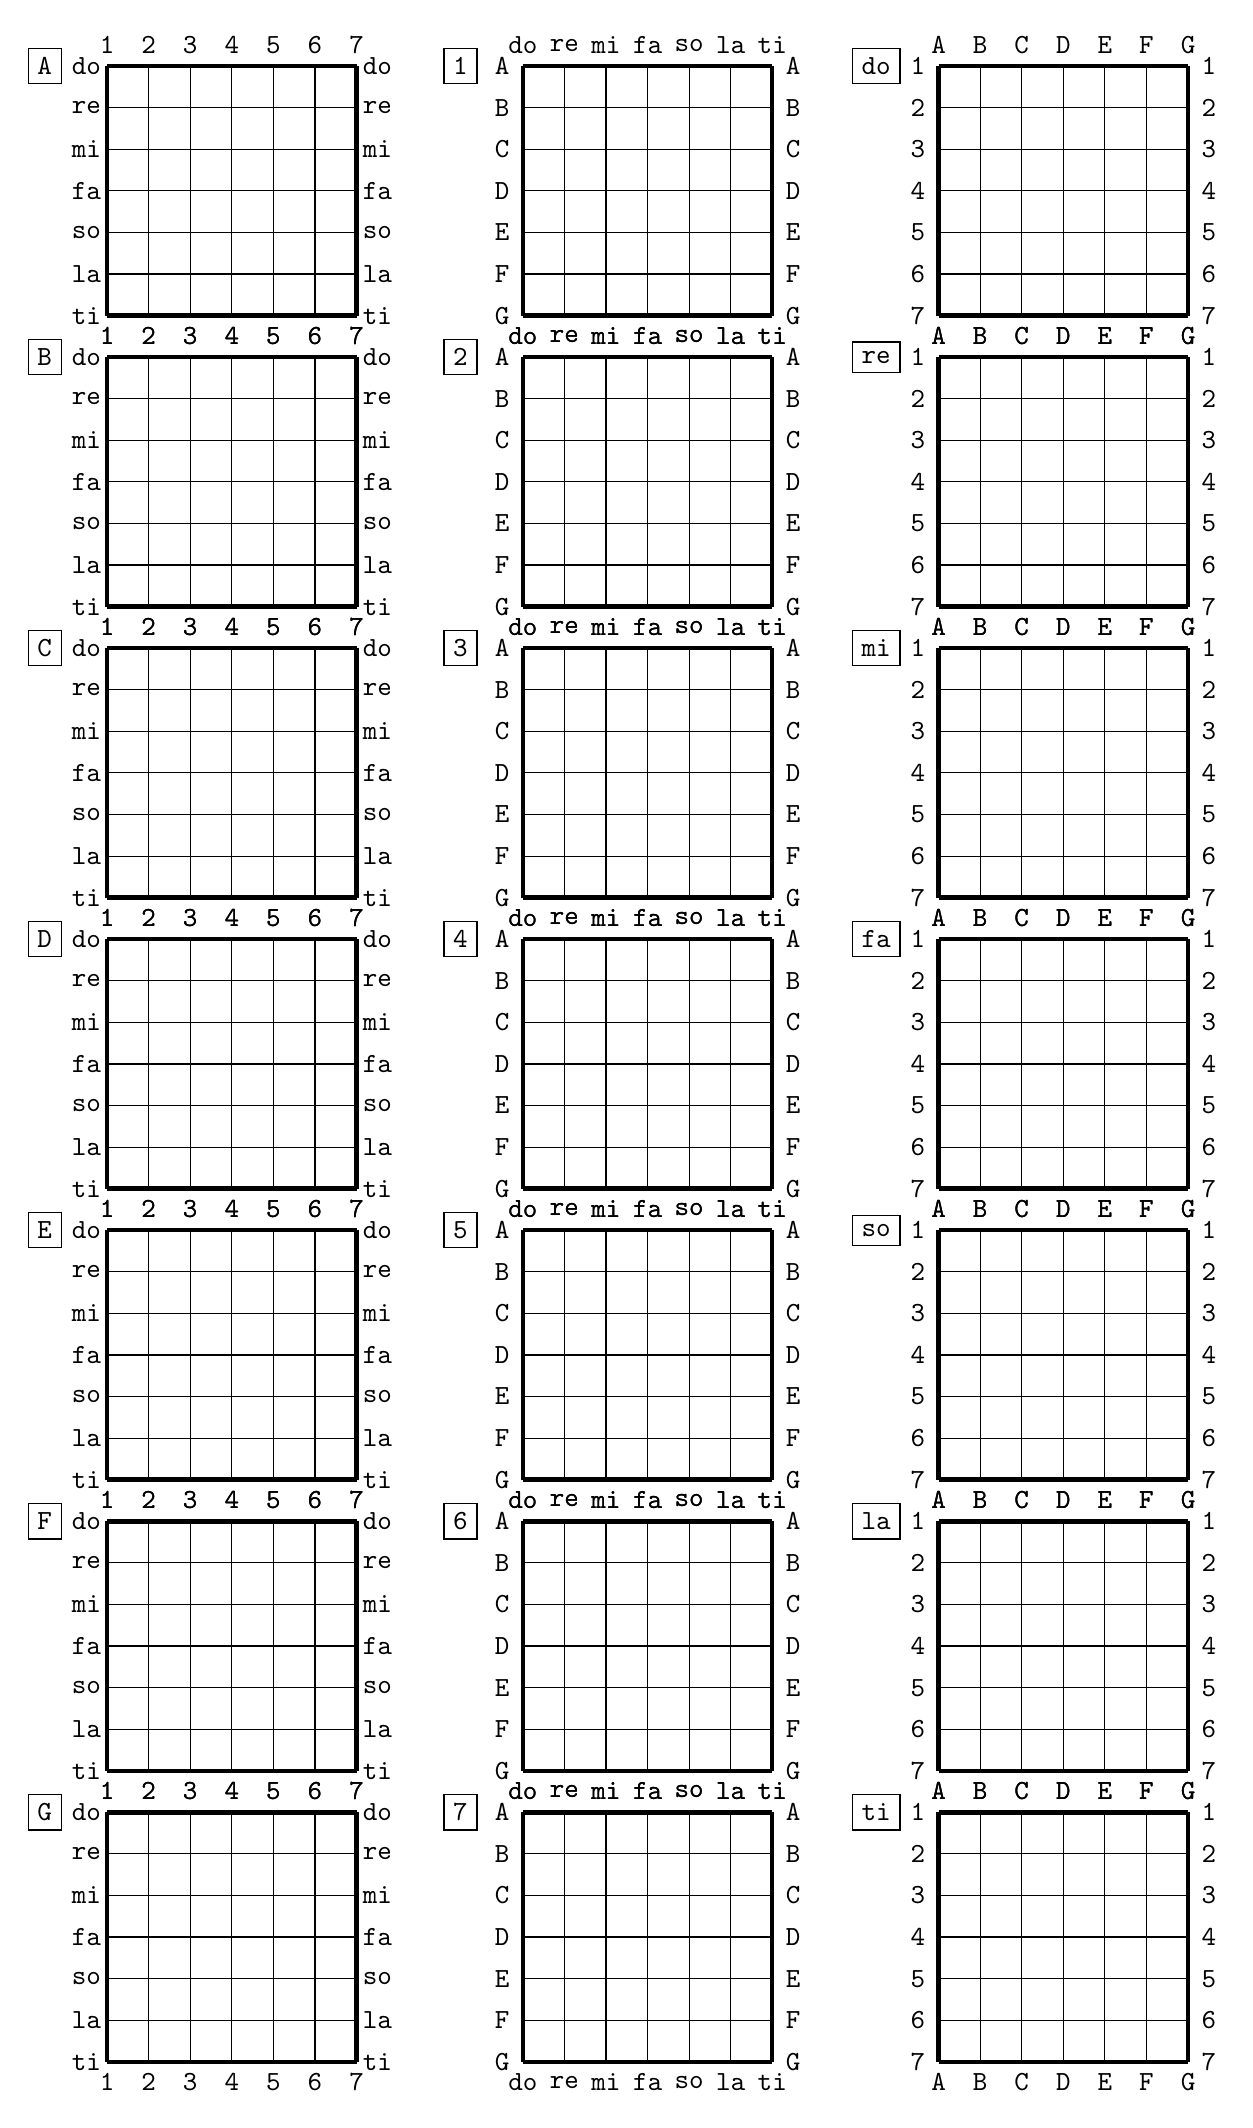
\begin{tikzpicture}
  %
  \newcommand\size{7}
  \begin{scope}[scale=0.66]

    \foreach \name [count=\i] in \letterlabels {
      \begin{scope}[scale=0.8,yshift=-\i*\size cm]

        \begin{scope}[shift={(-1.5,\size - 1)}]
          \node[draw] at (0,0) {\texttt{\name}};
        \end{scope}

        \upperboard{\size}

        \ifnum \i=\size
          \breakforeach
        \fi

      \end{scope}
    }

    \foreach \name [count=\i] in \numberlabels {
      \begin{scope}[scale=0.8,yshift=-\i*\size cm,xshift=10cm]

        \begin{scope}[shift={(-1.5,\size - 1)}]
          \node[draw] at (0,0) {\texttt{\name}};
        \end{scope}

        \numberboard{\size}

        \ifnum \i=\size
          \breakforeach
        \fi

      \end{scope}
    }

    \foreach \name [count=\i] in \musiclabels {
      \begin{scope}[scale=0.8,yshift=-\i*\size cm,xshift=20cm]

        \begin{scope}[shift={(-1.5,\size - 1)}]
          \node[draw] at (0,0) {\texttt{\name}};
        \end{scope}

        \lowerboard{\size}

        \ifnum \i=\size
          \breakforeach
        \fi

      \end{scope}
    }

  \end{scope}

\end{tikzpicture}
\end{center}

\end{document}
